\documentclass[tikz,border=10pt]{standalone}
\usetikzlibrary{arrows.meta}

\begin{document}
	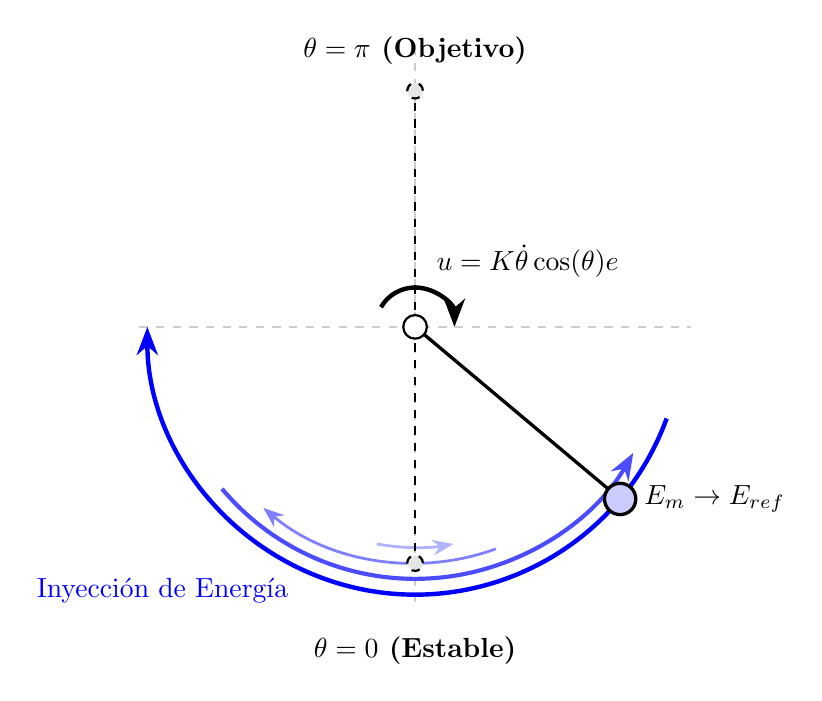
\begin{tikzpicture}[>=Stealth, thick]
		
		% --- CONFIGURACIÓN DE EJES ---
		\draw[dashed, gray!40] (0,-3.5) -- (0,3.5); % Eje vertical
		\draw[dashed, gray!40] (-3.5,0) -- (3.5,0); % Eje horizontal
		
		% --- TRAYECTORIA DE BALANCEO (CONCEPTUAL) ---
		% Ilustra el aumento gradual de energía descrito en el paper
		\draw[->, blue!30, line width=1pt] (260:2.8) arc (260:280:2.8);
		\draw[->, blue!50, line width=1pt] (290:3) arc (290:230:3);
		\draw[->, blue!70, line width=1.5pt] (220:3.2) arc (220:330:3.2);
		\draw[->, blue, ultra thick] (340:3.4) arc (340:180:3.4) node[midway, left, xshift=-25pt] {Inyección de Energía};
		
		% --- ESTADOS DEL PÉNDULO ---
		
		% 1. Posición Inicial (Estable / Downward position)
		% Se cambia gray!30 por dashed, black para que coincida con el objetivo[cite: 1]
		\draw[dashed, black] (0,0) -- (0,-3) node[circle, fill=black!10, draw=black, inner sep=2pt] {};
		\node[black, font=\bfseries, below] at (0,-3.8) {$\theta = 0$ (Estable)};
		
		% 2. Posición Intermedia (Durante el swing-up)
		\draw[line width=1.2pt] (0,0) -- (-40:3.4) node[circle, fill=blue!20, draw, inner sep=4pt] (mass) {};
		\node[black, right, xshift=5pt] at (mass) {$E_m \to E_{ref}$};
		
		% 3. Objetivo (Inestable / Upright position)[cite: 1]
		\draw[dashed, black] (0,0) -- (0,3) node[circle, fill=black!10, draw=black, inner sep=2pt] {};
		\node[black, font=\bfseries, above] at (0,3.2) {$\theta = \pi$ (Objetivo)};
		
		% --- ACCIÓN DE CONTROL (PAR u) ---
		% El par aplicado según la ley de control de energía[cite: 1]
		\draw[<-, ultra thick, black] (0.5,0) arc (0:150:0.5) node[midway, above right] {$u = K\dot{\theta}\cos(\theta)e$};
		
		% Pivot (Eje de rotación)
		\filldraw[fill=white] (0,0) circle (0.15);
		
	\end{tikzpicture}
\end{document}